\documentclass[10pt,letterpaper]{article}
\usepackage{graphicx}		% For the figures, allows scaling.
\usepackage{lmodern}		% Needed to generated good PDF
\usepackage{fullpage}
\usepackage{subfigure}
\usepackage{tabularx}
\usepackage{psfrag}
\usepackage{url}
\usepackage{hyperref}
\usepackage{color}

\newcommand{\jc}[1]{{#1}}

\title{ 15-441: Computer Networks\\ Project 2: TCP in The Wild\\ }

\author{TAs: Ranysha Ware (Ray)
             $<$\href{mailto:rware@andrew.cmu.edu }{rware@andrew.cmu.edu}$>$ \\
              Alex Bainbridge
             $<$\href{mailto:abainbri@andrew.cmu.edu}{abainbri@andrew.cmu.edu}$>$}
\date{}


\begin{document}

\maketitle

\section{Overview} 

In class, we have been talking about TCP, the default transport protocol on the Internet. TCP serves many purposes: it provides reliable, in-order delivery of bytes, it makes sure the sender does not send too fast and overwhelm the receiver (flow control), and it makes sure the sender does not send too fast and overwhelm the network (congestion control). It also aims to be fair: when multiple senders share the same link, they should receive roughly the same proportion of bandwidth.

In class, we discussed TCP Reno. A variant of TCP Reno, NewReno used to be the standard TCP on the Internet. But these are just one of many congestion control algorithms (CCAs). Companies use different TCPs depending on the context, for example, one TCP for data centers and another for serving web content.

If you are curious learn more about TCPs in the real world, here is are some fun CCAs to read about:
Microsoft and Google use very different approaches to TCP in their datacenters. DCTCP is a TCP for datacenters designed by Microsoft. TIMELY is a TCP for datacenters designed by Google.
For web content, the most common algorithm -- and the default in Linux servers -- is called Cubic. Akamai, the largest content distribution network in the world, uses a proprietary TCP called FastTCP.

In this project, you will demonstrate your understanding of the TCP basics by implementing TCP Reno. You will then use your own engineering skills to design a modern TCP for the datacenter, the Internet, or Earth to Moon communication.




\begin{table}[h]
\begin{center}
\begin{tabular}{l|l}
 \textbf{Date} & \textbf{Description} \\ \hline February 19 & Project
 released. \\ \jc{March 4} &
 \textbf{Checkpoint 1}: Data Serialization and transmission
 \\ \jc{March 22} &
 \textbf{Checkpoint 2}: TCP Reno implementation
 \\ \jc{March 29} & \textbf{Final Project Deadline by 11:59 P.M.} \\
\end{tabular}
\end{center}
\label{tab:duedate}
\end{table}



\section{CMU-TCP}
TCP is a network layer protocol that enables different devices to communicate. There are a variety of different TCP protocols such as Reno, New Reno, Cubic, and more. For this project we are focusing on Reno. As a reminder the basic setup of Reno is the following. \\

You have an initiator (client) and a listener (server). The listener is waiting to receive a connection from the initiator. After a connection is received, they perform a TCP handshake to initate the connection. Afterwards, they can perform read and writes to each other. From the application layer, reads and writes to the socket are buffered before being sent over the network. This means that multiple reads or writes might be combined into a single packet or the opposite, that a single read or write to a socket might be split into many packets.\\

In order to establish reliable data transfer, TCP has to manage lots of different variables and data structures. Here is an example of some of the details you'll need to track.\\

Let's say we have sockets A and B, and that socket A wants to start sending data to socket B. A will store the data in a buffer that it will pull from for sending packets. Socket A will then create packets using data from the buffer and send as many as it is allowed to send based on the congestion control algorithm used. As Socket B receives packets, it stores the data transmitted in a buffer. This buffer helps with maintaining the principle of in-order data transmission.  B sends ACKs as responses to A to notify A that various bytes have been received up to a certain point. B is also tracking the next byte requested by the application reading from the socket, and when it receives this byte, will forward as much data in order that it can to the applications buffer. For example, if B is looking for byte number 400, it will not write any other bytes into the application's buffer until it receives byte number 400. After receiving byte number 400, it will write in as many other bytes as it can. (If B had bytes 400-1000 then all  would be written to the application buffer at the time of receiving the packet with byte 400. As packets are ACK'd, socket A will release memory used for storing data as they no longer need to hold onto it. Finally either side can initiate closing the connection where the close handshake begins. \\

As both sides (initiator and listener) can both send and receive, you'll be tracking a lot of data and information. It's important to write down everything each side knows while writing your implementation and to utilize interfaces to keep your code module and re-usable. 

\section{Project specification}
\subsection{Background}

This project will consist of three checkpoints. The first checkpoint will have you build the basics of TCP: reliable, in-order delivery and flow control. In the second checkpoint, you will implement the Reno CCA and demonstrate to us that it is correct. In the third and final checkpoint, you will design and implement your own CCA for one of three scenarios: a datacenter, the Internet, or Earth to Moon communication.

\subsection{What are you actually turning in}
You are implementing the cmu\_tcp.h interface. Your code will be tested by us creating other C files that will utilize your interface to perform communications. The starter code has an example of how we might perform the tests, we have a client.c and server.c which utilize the sockets to send information back and forth. You can add additional helper functions to cmu\_tcp or change the implementation of the 4 core functions (socket, close, read and write), however you cannot change the function signature of the 4 core functions. Further, we will be utilizing grading.h to help us test your code. We may change any of the values for the variables present in the file to make sure you aren't hard coding anything. Namely, we will be fluctuating the packet length, and the initial window variables. \\

Additionally, for each checkpoint you will need to provide a graph showing the number of packets in flight (or unacked packets) vs time. We have provided you with a samplefile in the test directory that you can transfer and graph. We have also provided a python file called gen\_graph.py to help you generate the graph. It should be setup to monitor packets sent to and from the sender's perspective - you may need to change and update the gen\_graph.py script in order to provide a quality graph. 




\section{Checkpoint 1}
In this checkpoint, you will implement windowed transmission, where more than one packet can be ``on the wire" at the same time. You will start by extending a simple ``stop and wait" implementation that we provide.

\subsection{Learning Objectives}
With this section, you will learn to think about data packetization and reconstruction, TCP windowing, and packet retransmission. You will also continue to strengthen your C programming skills.

\subsection{Starter Code}
The following files have been provided for you to use:
\begin{itemize}
\item cmu\_packet.h: this file describes the basic packet format and header. You are not allowed to modify this file until the final submission! The scripts that we provide to help you graph your packet traces rely on this file being unchanged.
\item grading.h: these are variables that we will use to test your implementation, please do not make any changes here as we will be replacing it when running tests. 
\item server.c:  this is the starter code for the server side of your transport protocol. 
\item client.c: this is the starter code for the client side of your transport protocol.
\item cmu\_tcp.c: this contains the main socket functions required of your TCP socket including reading, writing, opening and closing. 
\item backend.c: this file contains the code used to emulate the buffering and sending of packets. This is where you should spend most of your time.
gen\_graph.py: Python script that takes in a pcap file and graphs your sequence numbers by time. 
\item cmu\_packet.h
All the communication between your server and client will use UDP as the underlying protocol. All packets will begin with the common header described in cmu\_packet.h as follows:
\begin{itemize}
    \item Course Number 		[4 bytes]
    \item Source Port 			[2 bytes]
    \item Destination Port 		[2 bytes]
    \item Sequence Number 		[4 bytes]
    \item Acknowledgement Number 	[4 bytes]
    \item Header Length		[2 bytes]
    \item Packet Length			[2 bytes]
    \item Flags				[1 byte]
    \item Advertised Window		[2 bytes]
    \item Extension length		[2 bytes]
    \item Extension Data		[You Decide]
\end{itemize}
\end{itemize}

All multi-byte integer fields must be transmitted in network byte order. ntoh, hton, and friends will be very important functions for you to call! All integers must be unsigned, and the course number should be set to 15441 (the scripts rely on this). You are not allowed to change any of the fields in the header, with the exception of the extension data which you may want to modify in Checkpoint 3. Additionally, plen cannot exceed 1400 in order to prevent packets from being broken into parts.

You can verify that your headers are sent correctly using wireshark or tcpdump. You can view packet data sent including the full Ethernet frames. When viewing your packet you should see something similar to the below image; in this case the payload starts at 0x0020. The course number - 15441- shows up in hex as 0x00003C51.\\
  
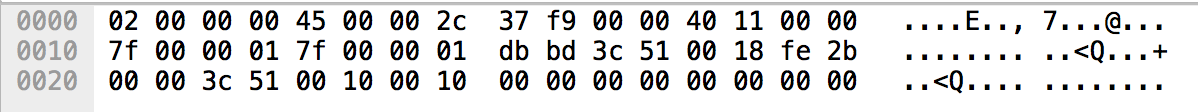
\includegraphics[scale=0.75]{sample_data.png}

\subsection{Checkpoint 1 Tasks }
\begin{enumerate}
    \item TCP Handshakes - Implement TCP start and end handshakes before data transmission starts and ends ~\cite{tcp-conn-state}. This should happen in the constructor and destructor for cmu\_socket. 
    \item Flow Control - You will notice that data transfer is very slow. That is because the starter code is using the Stop-and-Wait algorithm, transmitting one packet at a time! You can do much better by using a window of outstanding packets to send on the network. Extend the implementation to: 1) Change the sequence numbers and ACK numbers to represent the number of bytes sent and received (rather than segments) 2) Implement TCP's sliding window algorithm to send a window of packets and utilize the advertised window to limit the amount of data sent by the sender~\cite{sliding-window}. You do not need to implement Nagle's algortihm.
    \item RTT Estimation -  You will notice that loss recovery is very slow! One reason for this is the starter code uses a fixed retransmission timeout (RTO) of 3 seconds. Implement an adaptive RTO by estimating the RTT with Jacobson/Karels Algorithm or using the Karns/Partridge algorithm~\cite{rto-implementation}. 
    \item Duplicate ACK Retransmission -  Another reason loss recovery is slow is the starter code relies on timeouts to detect packet loss. One way to recover more quickly is to retransmit whenever you see triple duplicate ACKs. Implement retransmission on the receipt of 3 duplicate ACKs.
\end{enumerate}



\section{Checkpoint 2}
Once you have implemented the basics, you can add a Congestion Control Algorithm (CCA) to handle overloading in the network. You will implement TCP Reno, as discussed in class. Hence, the number of outstanding (unACKed) packets will now be be min(window size, congestion window size). You will have to demonstrate to us using traces of real connections that your TCP Reno implementation uses Additive Increase under normal operation, and Multiplicative Decrease under loss.

\subsection{Learning Objectives}
With this section, you will learn how TCP manages to maintain a view of the network state, as well as how the TCP state machine for congestion control works (shown below). Implementing TCP Reno will allow you to transfer data faster as you utilize more available bandwidth for data transmission. Additionally, fast recovery will allow you efficiently recover when packets have been lost. 


\subsection{Checkpoint 2 Tasks}
\begin{enumerate}
    \item Basics - Review and understand the TCP congestion control state machine in depth! \cite{state_machine}
    
    \item 
    Update the your code from Checkpoint 1 to add a new parameter, the congestion window: \texttt{cwnd}. The size of your sending window should now be the minimum of \texttt{cwnd} and the advertised window. You should additionally maintain that the total amount of data buffered for the application (unread data, both ordered and unordered bytes) should be less than \texttt{MAX\_NETWORK\_BUFFER}. 
    
    \item Congestion Control - Implement the slow start and congestion avoidance features of the state machine, this should make your implementation like TCP Tahoe. 
    
    \item Fast Recovery - Implement fast recovery, this should move your implementation from Tahoe to Reno. Note, you only need to implement TCP Reno, not TCP NewReno.
    
    \item Make sure to test your new features with many different network settings using \texttt{tcconfig}. You should transmit a large file again using your TCP implementation, like you did in Checkpoint 1, set the bandwidth small in relation to the size of your file (ex: transferring 100Mb file, 1Mbps bandwidth) and add packet loss (ex: 5\%) in order to see the TCP sawtooth pattern.
\\

\texttt{Here is a copy of the full state machine}\\
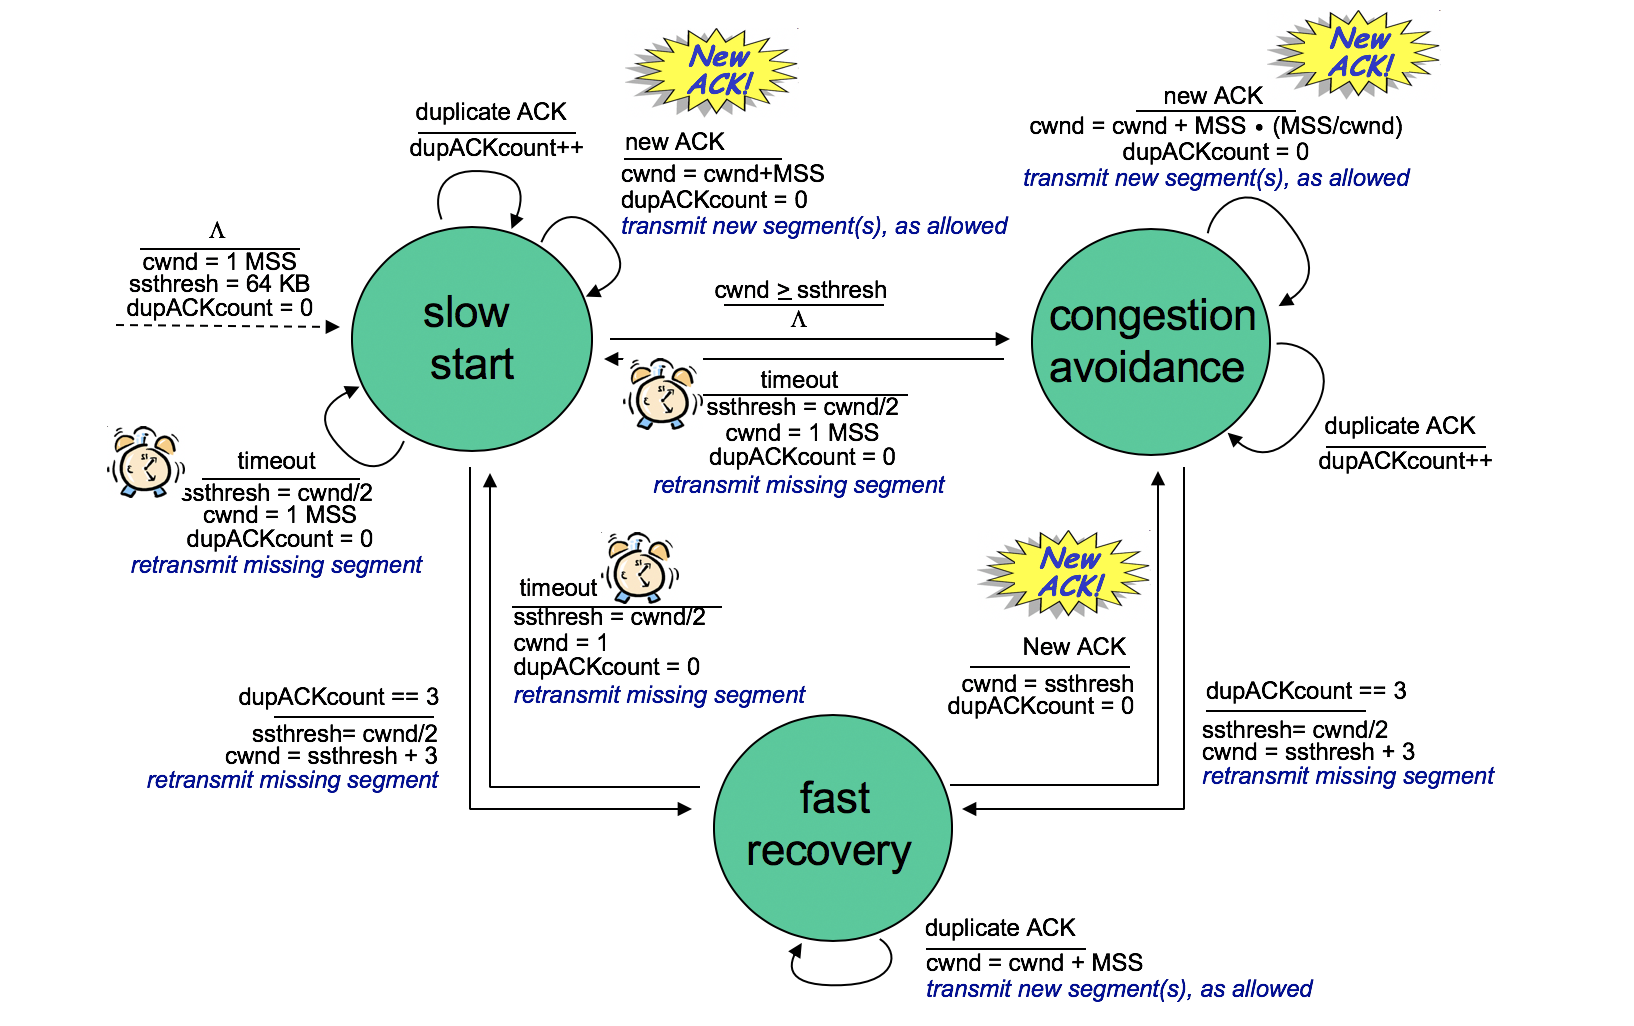
\includegraphics[scale=0.3]{image.png}

\end{enumerate}


Here are the values from \texttt{grading.h} you must use in your code for this checkpoint. We will test your code (and you should too!) by changing these values. All of these values are in bytes.

\begin{enumerate}
    \item \texttt{WINDOW\_INITIAL\_WINDOW\_SIZE}: Initial window size for slow start. In slow start, you should initially set \\ \texttt{cwnd} = \texttt{WINDOW\_INITIAL\_WINDOW\_SIZE}.
    \item \texttt{WINDOW\_INITIAL\_SSTHRESH}: \texttt{ssthresh} value for congestion control. In slow, start, you should initially set \texttt{ssthresh} = \texttt{WINDOW\_INITIAL\_SSTHRESH}.
    \item \texttt{MAX\_LEN}: Max packet length of any packet - including header. This value will not change and will always remain fixed.
    \item \texttt{MAX\_NETWORK\_BUFFER}: Maximum number of bytes that the TCP implementation can hold/buffer for the application. (This includes unread, ordered and unordered bytes received on the network, and received by the application). Thus, the size of your \texttt{sending\_buf} should be set to \texttt{MAX\_NETWORK\_BUFFER} and the size of  \texttt{received\_buf} should be set to \texttt{MAX\_NETWORK\_BUFFER}.
\end{enumerate}




\section{Checkpoint 3}
In checkpoint 3, you will improve your TCP implementation for one of three scenarios:
\begin{enumerate}
    \item Moon - For the moon, set loss rate to 30\%, 2.5 seconds of delay, and a max bandwith of 10 megabits per second. 
    \item Data Center - For the data center, set loss rate to 0.05\%, delay 0.1 seconds, and a max bandwith of 5 gigabits per second. 
    \item AWS Server to Client - For the server, set loss rate to 1\%, delay to 0.2 seconds, and a max bandwith of 50 megabits per second. 
\end{enumerate}

\noindent (A) Your first step is to {\it profile} your Reno implementation. Using your Reno implementation, transfer a 20MB file in your chosen scenario. How long does it take for the file transfer to complete? Consider Reno's design: what makes it slower than it could be? If the file transfer does not complete in a reasonable amount of town, why is this?

\noindent{\bf Deliverable:} In a file called {\bf designdiscussion.pdf}, turn in a graph of your Reno implementation running in your chosen scenario. Write at least two paragraphs describing what aspects of Reno's design make it perform less-well than it could in your chose scenario. 

\vspace{10pt}

\noindent (B) Your second step is to design a new congestion control algorithm. There is only one requirement: that your new implementation finishes at least 10\% faster than your original implementation (or, if your first implementation did not complete within 20 minutes, that your new implementation does complete in that amount of time). One way to pass this step is to implement TCP Cubic or TCP BBR, but you may also design your own algorithm.

\noindent{\bf Deliverable:} In the same file called {\bf designdiscussion.pdf}, provide a graph of your new algorithm running in your chosen scenario. Answer the following questions:
\begin{enumerate}
    \item Describe your new algorithm to someone else who needs to implement it too. How does it work? What is the `state machine' to update your new algorithm?
    \item How long does it take for your new CCA to transfer a 20MB file? How long does it take your Reno implementation?
    \item What is different about your new CCA that makes it perform better than Reno in tranferring 20MB files?
    \item How long does it take for your new CCA to transfer a 3MB file? How long does it take your Reno implementation?
    \item Explain why one algorithm performs better than the other, or why they perform equally.
\end{enumerate}

\vspace{10pt}

\noindent (C) (Optional) In this step you will tune your algorithm for competition! The TAs will test the top-5 fastest algorithms by running them in a real datacenter (AWS or Google CLoud), over the real wide area (from CMU to AWS or Google Cloud), or to the (simulated, sorry) Moon.

We will run two tests. First, we will transfer one 20MB file. We will measure the {\it average goodput} (the number of useful bytes transferred over time) from when we start sending to when the file transfer completes. Second, we will transfer four 20MB files simultaneously. We will measure each connection's average goodput and compute {\it Jain's Fairness Index.} Your total score will be the goodput for the single connection test, multiplied by Jain's Fairness Index for the four-connection test.

You can run these tests yourself and tune your code. There will be one prize for each of the three categories. We have some credits for Google Cloud and AWS if you would like to test over the real scenarios, please email staff-441@cs.cmu.edu to request credits.


 

\section{Testing Your Code}

\section{Hand-In}
\label{sec:handin}

As in Project 1, code submission for checkpoint and the final deadline will be done 
through {Autolab (autolab.cs.cmu.edu).}
Every checkpoint will be a git tag in the code repo. To create a tag, run
\[
\texttt{git tag -a checkpoint-\textit{<num>} -m \textit{<message>} [\textit{<commit hash>}]}
\]
with appropriate checkpoint number and custom message filled in. (Put whatever
you like for the message --- git won't let you omit it.) The optional commit
hash can be used to specify a particular commit for the tag; it you omit it,
the current commit is used. 
\noindent For the checkpoint, you will be expected to have a working Makefile, and 
whatever source needed to compile a working binary.  \textbf{Checkpoints that do not compile will
NOT be graded.}  
{To submit your code, make a tarball file of your repo after you tag it. Then login to autolab website,
choose \texttt{15-441: Computer Networks (S19) -> project2cp<{\it N}>}, and then upload your tarball.}
The submitted tarball should contain a directory named \texttt{15-441-project-2}, which has 
the following files that implement all required functionality:
\begin{itemize}
\item Makefile:  Make sure all the variables and paths are set correctly such 
that your program compiles in the hand-in directory. Running \texttt{make test} should run your testing code.
%Makefile should build the executable ``peer'' that runs on the andrew machines.
\item All of your source code files and test files. (files ending in .c, .h, etc. only, no .o files and no executables)
\item readme.txt: File containing a thorough description of your design and implementation. If you use any additional packet headers, please document them 
here. 
\item tests.txt: File containing documentation of your test cases and any known issues you have.

\item submit.pcap: Your PCAP submission file from running the functionality code in server.c and client.c from the starter code (for a larger file transfer). 

\item graph.pdf: Your graph of the currently unacked packets in flight vs time computed from submit.pcap. 
\end{itemize}

If you have an issue with uploading large files to Autolab, follow these directions: \url{https://piazza.com/class/jqfmjnmztjt4rv?cid=792}.






\begin{thebibliography}{1}
\bibitem{tcp-conn-state}
TCP connection establishment and termination: \\ \url{https://book.systemsapproach.org/e2e/tcp.html#connection-establishment-and-termination}

\bibitem{sliding-window}
TCP sliding window: \\
\url{https://book.systemsapproach.org/direct/reliable.html#sliding-window} \\
\url{https://book.systemsapproach.org/e2e/tcp.html#sliding-window-revisited}

\bibitem{rto-implementation} 
Adaptive retransmission: \\ \url{https://book.systemsapproach.org/e2e/tcp.html#adaptive-retransmission}

\bibitem{tc}
TCConfig: \url{https://github.com/thombashi/tcconfig}

\bibitem{tshark}
tshark: \url{https://www.wireshark.org/docs/man-pages/tshark.html}

\bibitem{wireshark-dissector}
Creating a wireshark dissector in Lua: \url{https://mika-s.github.io/wireshark/lua/dissector/2017/11/04/creating-a-wireshark-dissector-in-lua-1.html}

\bibitem{tcpdump}
tcpdump: \url{https://linux.die.net/man/8/tcpdump}

\bibitem{wireshark-plugin}
Wireshark plugin folder: \url{https://www.wireshark.org/docs/wsug_html_chunked/ChPluginFolders.html}

\bibitem{vagrant}
Vagrant: \url{https://www.vagrantup.com/intro/getting-started/index.html}

\bibitem{virtualbox}
VirutalBox:  \url{https://www.virtualbox.org/}

\bibitem{pytest}
pytest: \url{https://docs.pytest.org/en/latest/}

\bibitem{state_machine}
TCP Congestion Control: \url{https://intronetworks.cs.luc.edu/current/html/reno.html#tcp-reno-and-congestion-management}

\end{thebibliography}




\end{document}
